\documentclass[hyperref=colorlinks]{beamer}
\mode<presentation>
\usetheme{iclpt}
\setbeamertemplate{navigation symbols}{}
\setbeamertemplate{headline}{
  \begin{beamercolorbox}[leftskip=.2cm,rightskip=.2cm,topskip=.2cm,ht=1.1cm,dp=0.1cm,wd=\textwidth]{institute in head/foot}
    
\includegraphics[height=1cm]{icl.pdf}
    \hfill
%    \includegraphics[height=1cm]{../Pics/ATLAS-Logo-Square-Blue-RGB.png}
%    
\includegraphics[height=1cm]{../Pics/CMS-Color.pdf}
    
\includegraphics[height=1cm]{TalkPics/t2k_logo_large.png}

%??put t2k logo here
  \end{beamercolorbox}
}
\setbeamertemplate{footline}{
  \begin{beamercolorbox}[ht=.35cm,dp=0.2cm,wd=\textwidth,leftskip=.3cm]{author in head/foot}%
    \begin{minipage}[c]{5cm}%
      \usebeamerfont{author in head/foot}
      \insertshortauthor 
      \insertshorttitle
    \end{minipage}\hfill%
    \hfill
    \insertframenumber{} / \ref{lastframe}
    %\hfill
    \begin{minipage}{6cm}
      \hfill
      %\insertshorttitle
    \end{minipage}
  \end{beamercolorbox}%
}

\definecolor{beamer@icdarkblue}{RGB}{0,51,102}
\definecolor{beamer@icmiddleblue}{RGB}{0,82,150} 
\definecolor{beamer@iclightblue}{RGB}{200,212,232}
\definecolor{beamer@icmiddlered}{RGB}{204,51,0}
\definecolor{beamer@iclightred}{RGB}{232,212,32}

\usepackage{tikz}
\usetikzlibrary{arrows,shapes,backgrounds}
\usepackage{color}
\usepackage{tabularx,colortbl}
\usepackage{graphicx}
\usepackage{pdfpages}
\usepackage{feynmp}
\usepackage{rotating}
\usepackage{moresize}
\usepackage{slashed}
\usepackage{xcolor,colortbl}
\DeclareGraphicsRule{*}{mps}{*}{}
\hypersetup{colorlinks=false}

\title[MaCh3 status and plans]{\vspace{-0.2cm} MaCh3 status and plans}
\author[P. Dunne]{Patrick Dunne - Imperial College London \\ for the MaCh3 group}
\titlegraphic{
  \vspace{-0.4cm}
}
\date{}
\begin{document}
\tikzstyle{every picture}+=[remember picture]
\tikzstyle{na} = [baseline=-.5ex]
\begin{fmffile}{t2ktemplatefeyndiags}


  %TITLE PAGE
  %20 mins + 5 questions
  \section{Title}
  \begin{frame}
    \titlepage
  \end{frame}

  \begin{frame}
    \frametitle{Overview}
    \begin{block}{}
        \scriptsize
        \begin{itemize}
        \item Le\"ila updated on Run 1-7 5 sample status
        \item Preparation for main summer analysis
        \item New things we're working on
      \end{itemize}
    \end{block}
  \end{frame}

  \begin{frame}
    \frametitle{Preparations for the summer: Analysers and baseline}
    \begin{itemize}
    \item Planned baseline analysis is 5 sample+ND280 joint fit with new Xsec parameterisation
    \item Le\"ila, Clarence and Patrick (me) will be the main analysers for this
    \item[-] Le\"ila has to graduate at some point this summer
    \item[-] We also have Elder and Kirsty in the group able to help
    \end{itemize}
  \end{frame}

  \begin{frame}
    \frametitle{Preparations for the summer: Framework}
    \begin{itemize}
    \item Turnaround from final inputs to results is about 1 week each for Asimov fits and data fits
    \item Clarence has made some improvements to code:
    \item[-] Multi-threaded to improve speed
    \item[-] Now easier to add new parameterisations to ND280
    \end{itemize}
  \end{frame}

  \begin{frame}
    \frametitle{Preparations for the summer: New Xsec parametrisation}
    \begin{itemize}
    \item Parameters are implemented in our ND280 (Clarence) and SK (Kirsty) code to the extent they're final
    \item[-] BeRPA implemented event-by-event already
    \item I'm waiting for freeze of parameters for spline production and SK implementation of spline parameters (see other talk)
    \end{itemize}
  \end{frame}

  \begin{frame}
    \frametitle{fitQun CC1$\pi$: Elder}
    \begin{itemize}
    \item Working on adding fitQun numu pion ring samples
    \item Aiming for stats only analysis in the next few weeks
    \item Will then add FSI+SI covariance matrix (with current implementation) as a conservative approach
    \item Also, working on preparing splines for this sample
    \item Red: unoscillated, Blue: oscillated
    \end{itemize}
    \centering
    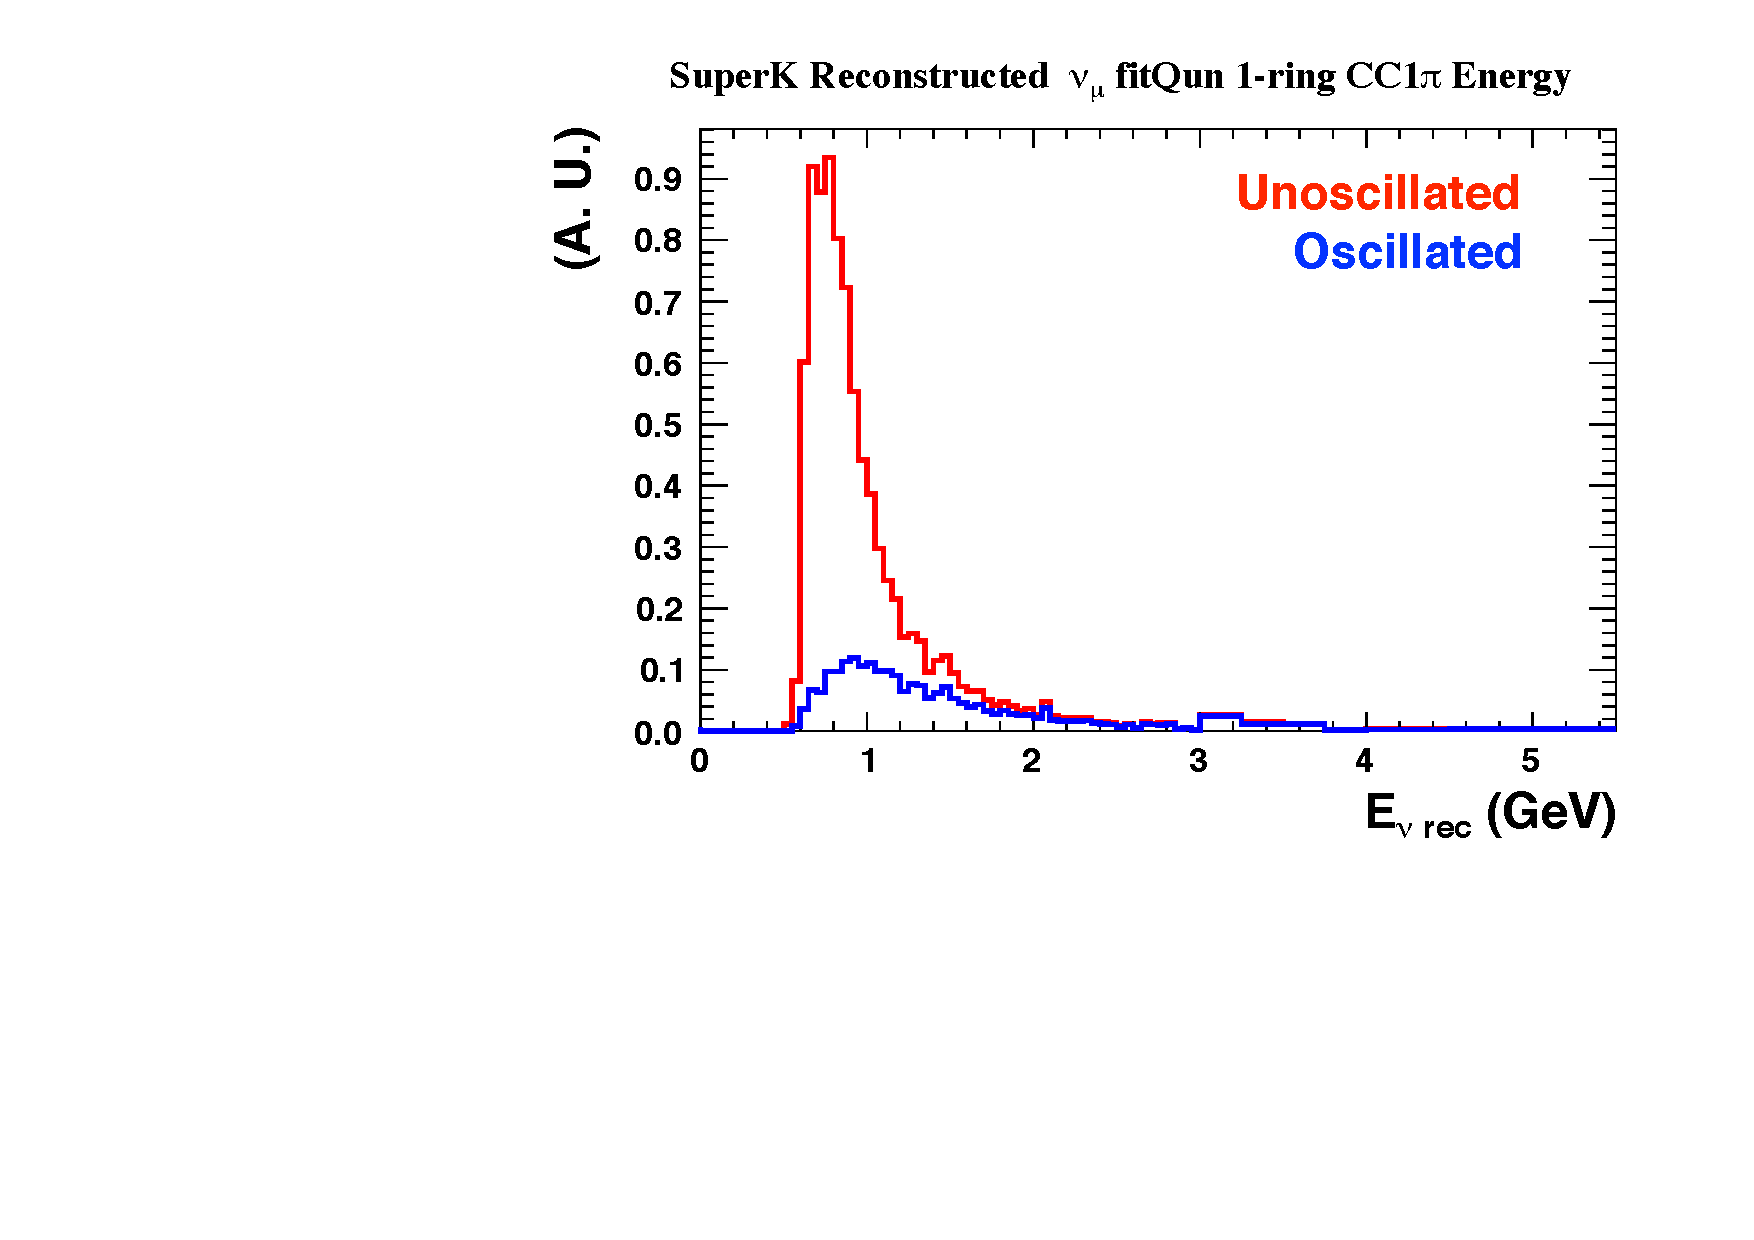
\includegraphics[width=.5\textwidth]{TalkPics/MaCh3update_070217/fitqun_1pi_elder_forPatrick.pdf}
  \end{frame}

  \begin{frame}
    \frametitle{Continuous $\beta$: Kirsty}
    \begin{itemize}
    \item Take $\beta$ from $\bar{\nu}_{e}$ appearance analysis and allow to be continuous
    \item Have run Asimov's (shown today set 1 wRC)
    \end{itemize}
    \centering
    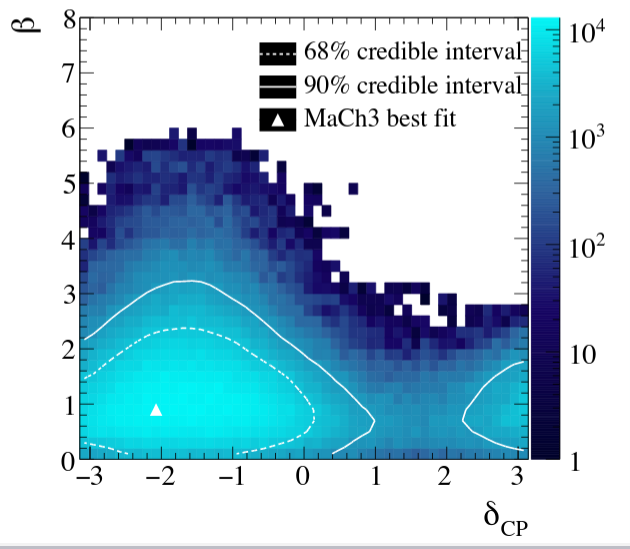
\includegraphics[width=.5\textwidth]{TalkPics/MaCh3update_070217/betadcp_asimov1wrc.png}
  \end{frame}

  \begin{frame}
    \frametitle{Continuous $\beta$: Kirsty}
    \begin{itemize}
    \item Take $\beta$ from $\bar{\nu}_{e}$ appearance analysis and allow to be continuous
    \item Have run Asimov's (shown today set 1 wRC)
    \item nb lower rightmost point is $\delta_{CP}=-\pi/2$
    \end{itemize}
    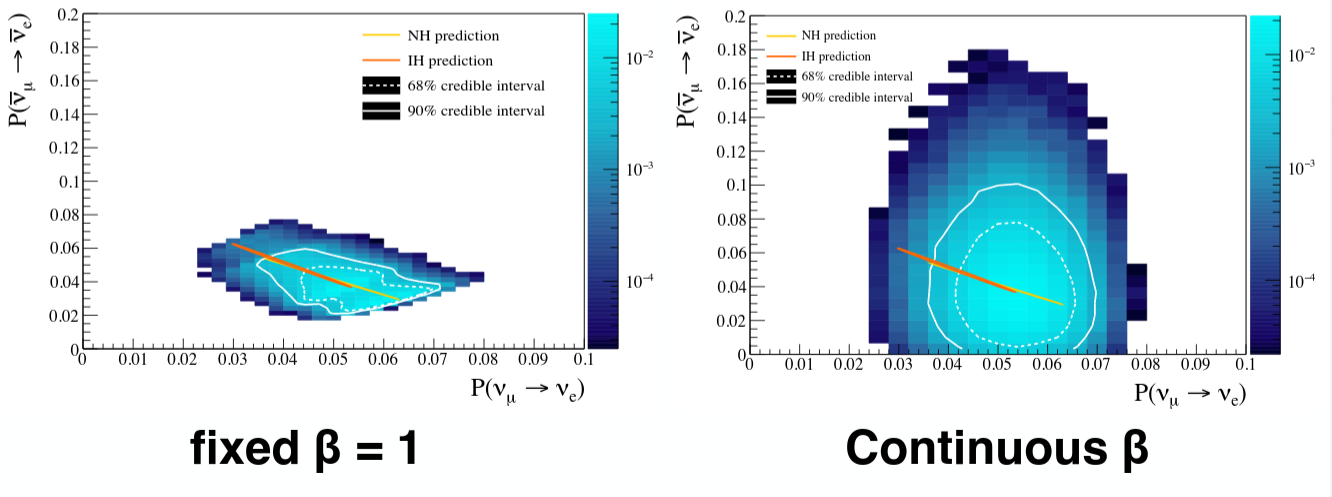
\includegraphics[width=\textwidth]{TalkPics/MaCh3update_070217/biprob_asimov1wrc.png}
  \end{frame}

  \begin{frame}
    \frametitle{2D $\nu_{\mu}$ studies: Me}
    \begin{itemize}
    \item Looking at finding a working $E_{rec}-\theta$ binning for 2D $\nu_{\mu}$
    \item Difficult to capture oscillation dip without very large number of bins
    \item Very preliminary kinematic plots shown here
    \end{itemize}
    \centering
    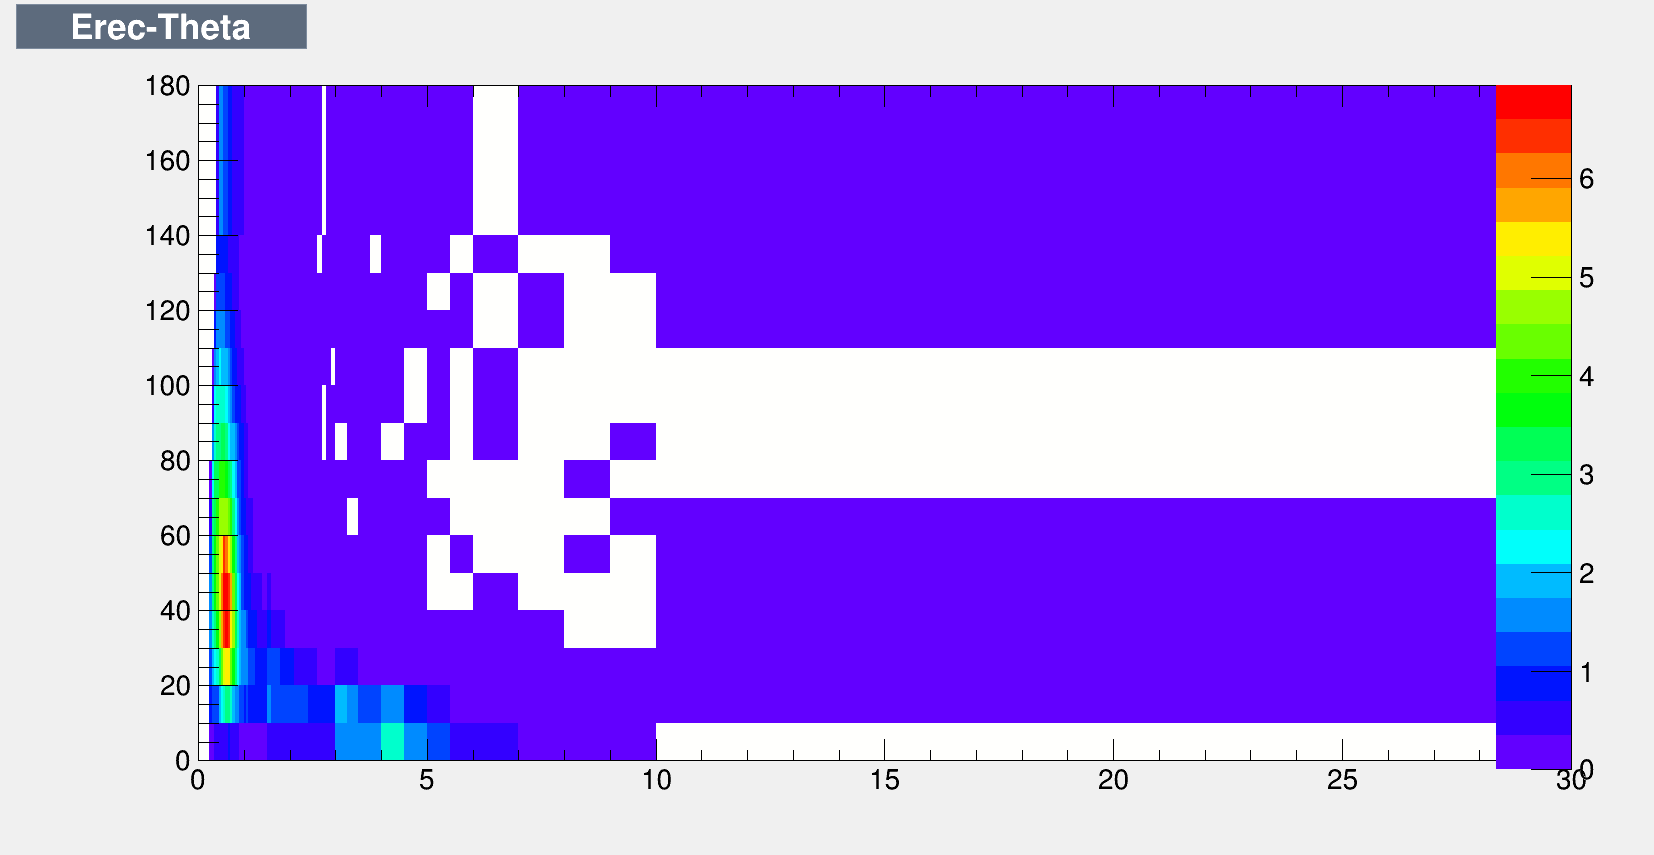
\includegraphics[width=.5\textwidth]{TalkPics/MaCh3update_070217/numu2dfullrange.png}
    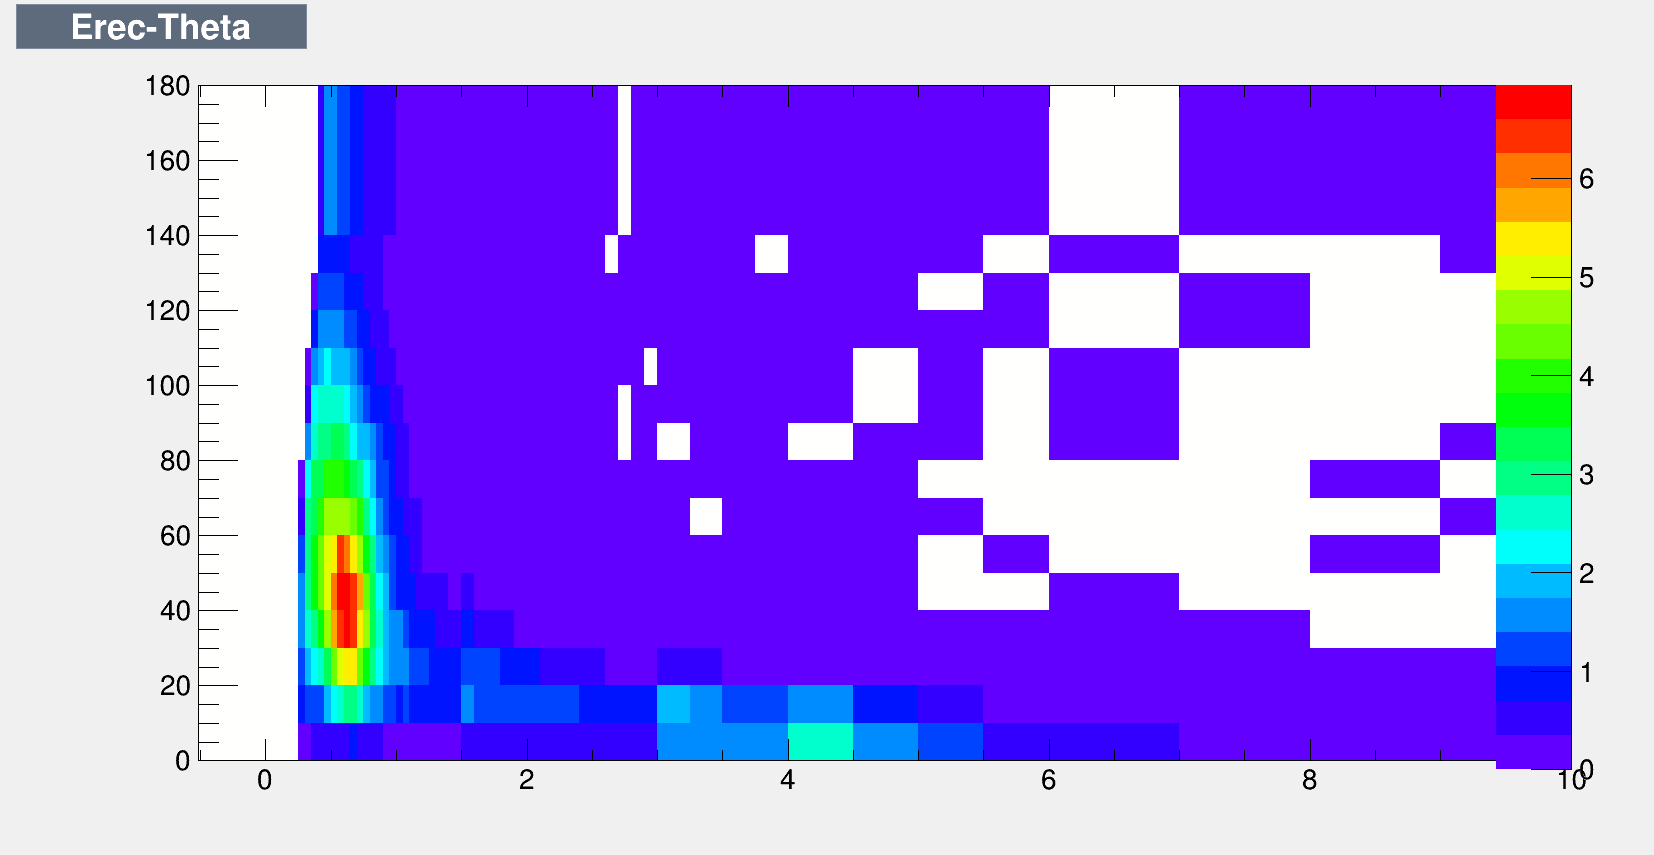
\includegraphics[width=.5\textwidth]{TalkPics/MaCh3update_070217/numu2dzoom.png}
  \end{frame}

  \begin{frame}
    \frametitle{ND280: Clarence}
    \begin{itemize}
    \item For summer: ready subject to last minute changes in Xsec parameterisation
    \item For future hopefully moving to psyche 3 at end of summer
    \item[-] Will allow $\nu_{e}$ and 4$\pi$ samples to be added
    \item[-] Dedicated person for this effort in BANFF now (Pierre Lasorak)
    \end{itemize}
  \end{frame}
  
  \begin{frame}
    \frametitle{Sterile search: Tarak}
    \begin{itemize}
    \item Plan to implement ND280 $\nu_{\mu}$ disappearance analysis with P6 and compare to previous analysis (based on P5)
    \item Have implemented 2 flavour oscillation weights
    \item Working to incorporate this into the Markov Chain 
    \item[-] Was planning ot use BANFF-like approach for cross-section parameters
    \item Significant effort recommended by NIWG convenors to implement a satisfactory cross-section model \textcolor{beamer@icmiddleblue}{\hyperlink{http://www.t2k.org/asg/xsec/meetings/2017/niwg-premeetings-febr2017/niwg-NDOAmodel}{see here}}
    \item Plan to have preliminary sensitivity studies with the recommended cross section model by Summer
    \end{itemize}
  \end{frame}


  \begin{frame}
    \frametitle{Conclusions}
    \label{lastframe}
    \begin{block}{}
      \begin{itemize}
      \item On track for Summer analysis
      \item[-] Ready for new Xsec parameterisation when it arrives
      \item[-] Framework is stable
      \item Several interesting new studies in progress
      \item[-] New samples at SK and ND280, continuous beta etc.
      \end{itemize}
    \end{block}
  \end{frame}

  %Backup goes here
  

\begin{frame}
  \centering
  \huge \textcolor{beamer@icmiddleblue}{Backup}
\end{frame}

%Add NH, IH and biprob prediction from Davide plots that Kirsty sent
\begin{frame}
  \frametitle{Continuous beta}
  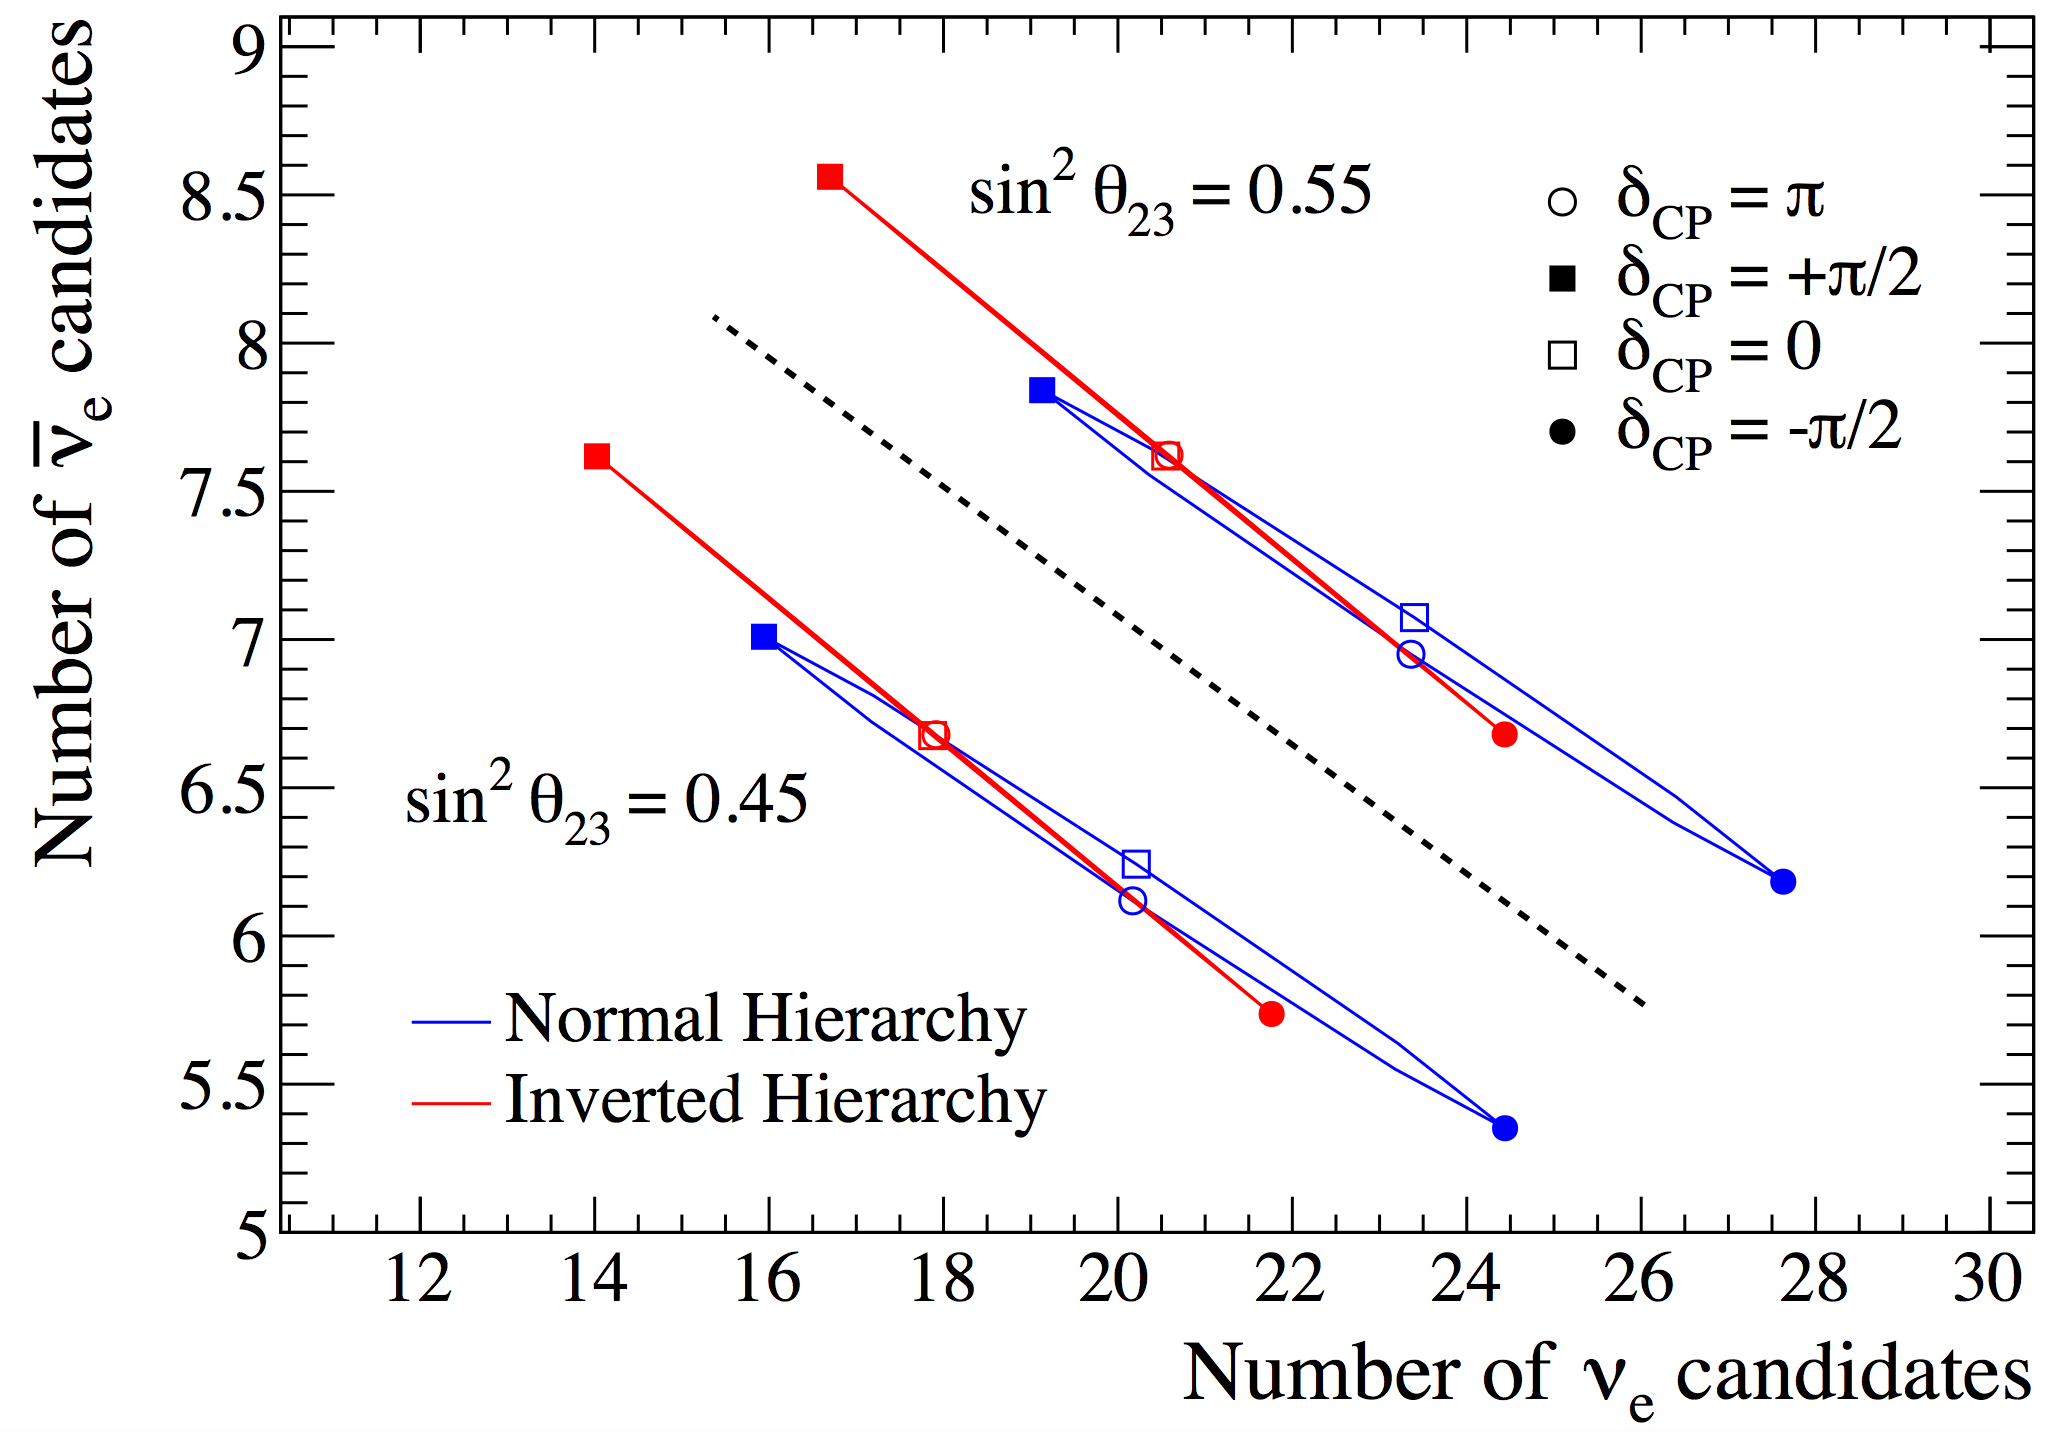
\includegraphics[width=\textwidth]{TalkPics/MaCh3update_070217/biprobpred.png}
\end{frame}

\begin{frame}
  \frametitle{Continuous beta}
  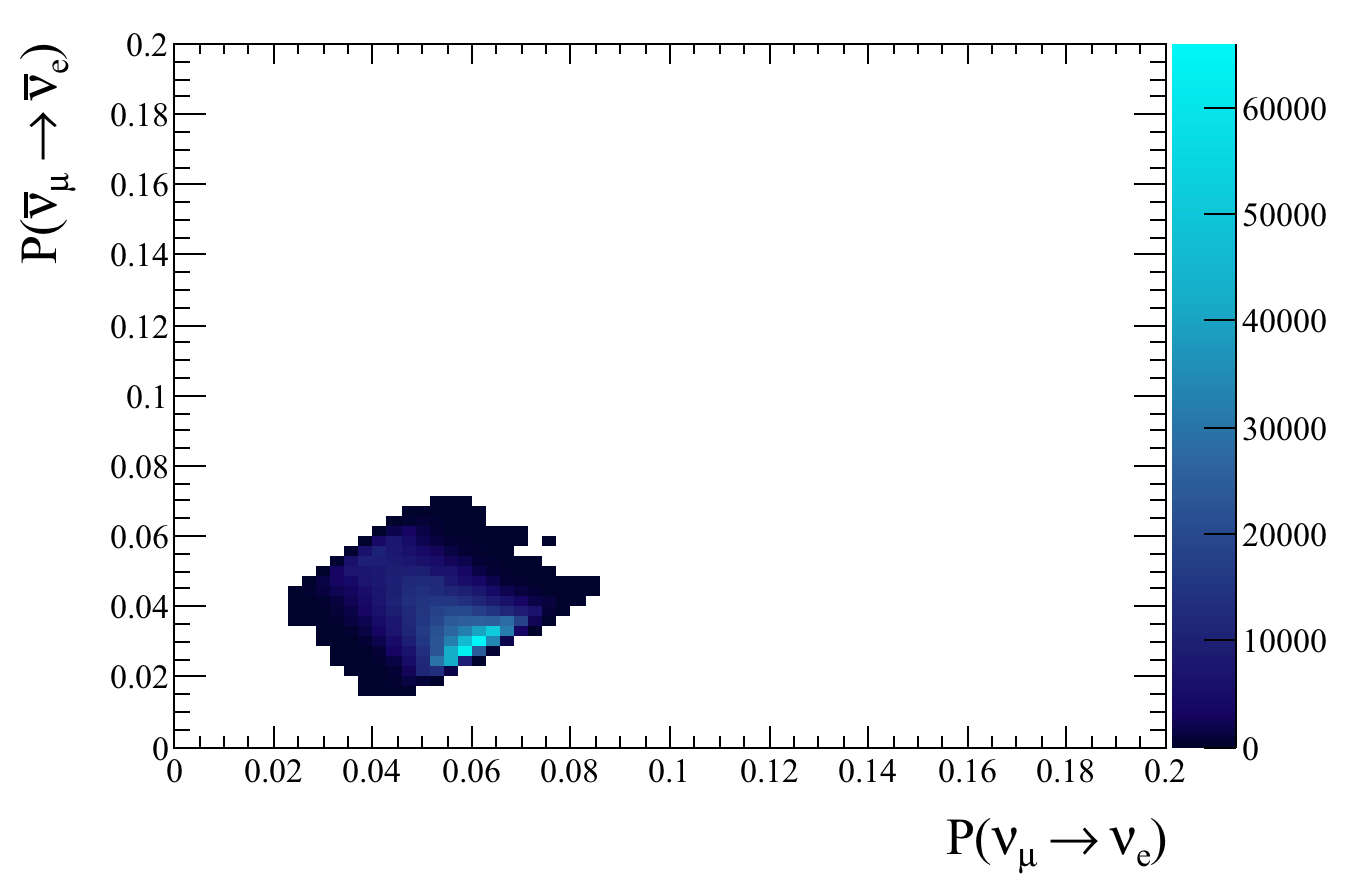
\includegraphics[width=.5\textwidth]{TalkPics/MaCh3update_070217/NHbiprob.png}
  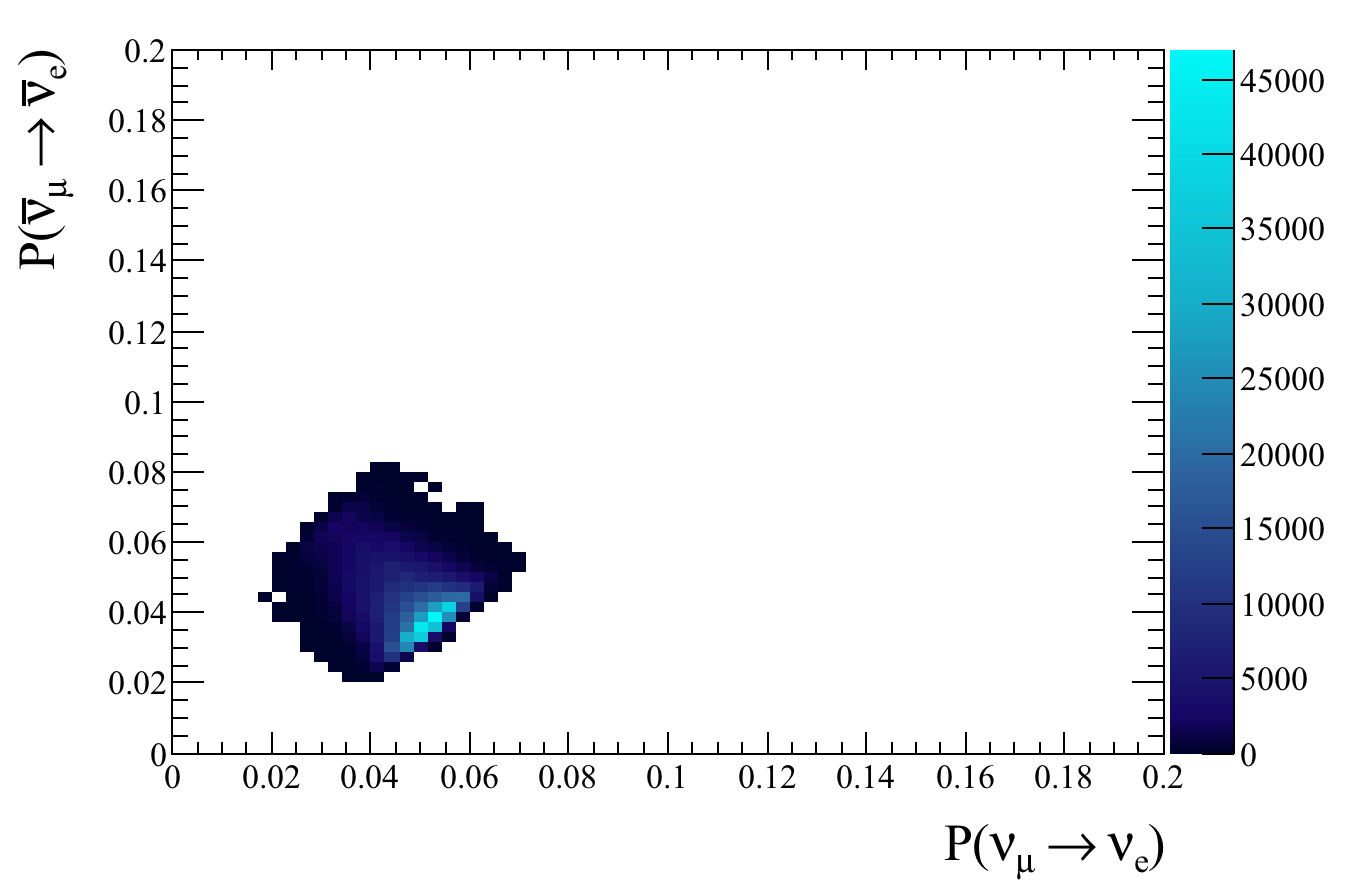
\includegraphics[width=.5\textwidth]{TalkPics/MaCh3update_070217/IHbiprob.png}
\end{frame}

\end{fmffile}
\end{document}
